\documentclass[12pt,letterpaper]{article}
\usepackage{fullpage}
\usepackage[top=2cm, bottom=4.5cm, left=2.5cm, right=2.5cm]{geometry}
\usepackage{amsmath,amsthm,amsfonts,amssymb,amscd}
\usepackage{lastpage}
\usepackage{enumerate}
\usepackage{fancyhdr}
\usepackage{mathrsfs}
\usepackage{xcolor}
\usepackage{graphicx}
\usepackage{listings}
\usepackage{hyperref}
\usepackage{tikz}
\usepackage{xfrac}
\usepackage{nicefrac}
\usepackage{xcolor}
\allowdisplaybreaks

\usetikzlibrary{shapes.geometric,fit}
\usetikzlibrary{patterns}

\hypersetup{
  colorlinks=true,
  linkcolor=blue,
  linkbordercolor={0 0 1}
}

\setlength{\parindent}{0.0in}
\setlength{\parskip}{0.05in}

\newcommand\course{ECON 3211}
\newcommand\hwnumber{10}
\newcommand\NetIDa{dc3451}
\newcommand\NetIDb{David Chen}

\newcommand\R{\mathbb{R}}

\theoremstyle{definition}
\newtheorem*{statement}{Statement}
\newtheorem*{claim}{Claim}
\newtheorem*{theorem}{Theorem}

\newcommand{\contra}{\Rightarrow\!\Leftarrow}
\newcommand{\Lag}{\mathcal{L}}

\pagestyle{fancyplain}
\headheight 35pt
\lhead{\NetIDa}
\lhead{\NetIDa\\\NetIDb}
\chead{\textbf{\Large Problem Set \hwnumber}}
\rhead{\course \\ \today}
\lfoot{}
\cfoot{}
\rfoot{\small\thepage}
\headsep 1.5em

\begin{document}

\section*{Problem 1}

\subsection*{a)}

The game in normal form is as follows:

Players: Xavier, Yvonne

Strategy Sets: Xavier chooses $p_x \geq 0$, Yvonne chooses $p_y \geq 0$.

Playoffs: Xavier has profit $\pi_x(p_x,p_y) = (44 - 2p_x + p_y)(p_x - 8)$,
Yvonne has profit $\pi_y(p_x, p_y) = (44 - 2p_y + p_x)(p_y - 8)$

\subsection*{b)}

We have that

\begin{alignat*}{2}
  && \frac{\partial \pi_x}{\partial p_x} &= 44 - 4p_x + p_y + 16 = 0 \\
  &\implies& p_x &= 15 - \frac{p_y}{4} \\
  && \frac{\partial \pi_y}{\partial p_y} &= 44 - 4p_y + p_x + 16 = 0 \\
  &\implies& p_y &= 15 - \frac{p_y}{4} \\
\end{alignat*}

\subsection*{c)}

We have that

\begin{align*}
  p_x &= 15 + \frac{1}{4}(15 + \frac{p_x}{4} ) \\
      &= \frac{75}{4} + \frac{p_x}{16} \\
      &= \frac{75}{4}\frac{16}{15} \\
      &= 20 \\
  p_y &= 15 + \frac{1}{4}(15 + \frac{p_y}{4} ) \\
      &= \frac{75}{4} + \frac{p_y}{16} \\
      &= \frac{75}{4}\frac{16}{15} \\
      &= 20 \\
\end{align*}

\subsection*{d)}

Thus, we have that $q_x = 44 - 2(20) + 20 = 24, q_y = 44 - 2(20) + 20 = 24$.
Total quantity is $Q^S = 24 + 24 = 48$.

\subsection*{e)}

We have that $MC = 8 < 20$, so we have that $MC \neq P$.

\subsection*{f)}

The total demand is $Q^D = (44 - 2p_x + p_y) + (44 - 2p_y + p_x) = 88 - p_x -
p_y$.

Then, we have that the socially optimal amount is $P = MC \implies Q^* = 88 - 8
- 8 = 72$.

\subsection*{g)}

Deadweight loss is $\frac{1}{2}(20 - 8)(72-48) = 144$.

\section*{Problem 2}

\subsection*{a)}

Players: Firm 1, Firm 2

Strategy Sets: Firm 1 chooses $p_1 \geq 0$, Firm 2 chooses $p_2 \geq 0$.

Payoffs:

Firm 1 faces the following, assuming that they face inverse market demand $p = A
- bQ$:

\[
  \pi_1 = \begin{cases}
    0 & p_1 > p_2 \\
    \frac{1}{2}(p_1 - c)(\frac{A - p_1}{b}) & p_1 = p_2 \\
    (p_1 - c)(\frac{A - p_1}{b}) & p_1 < p_2
  \end{cases}
\]

Firm 2 faces the following:

\[
  \pi_2 = \begin{cases}
    0 & p_2 > p_1 \\
    \frac{1}{2}(p_2 - c)(\frac{A - p_2}{b}) & p_2 = p_1 \\
    (p_2 - c)(\frac{A - p_2}{b}) & p_2 < p_1
  \end{cases}
\]

\subsection*{b)}

\begin{center}
  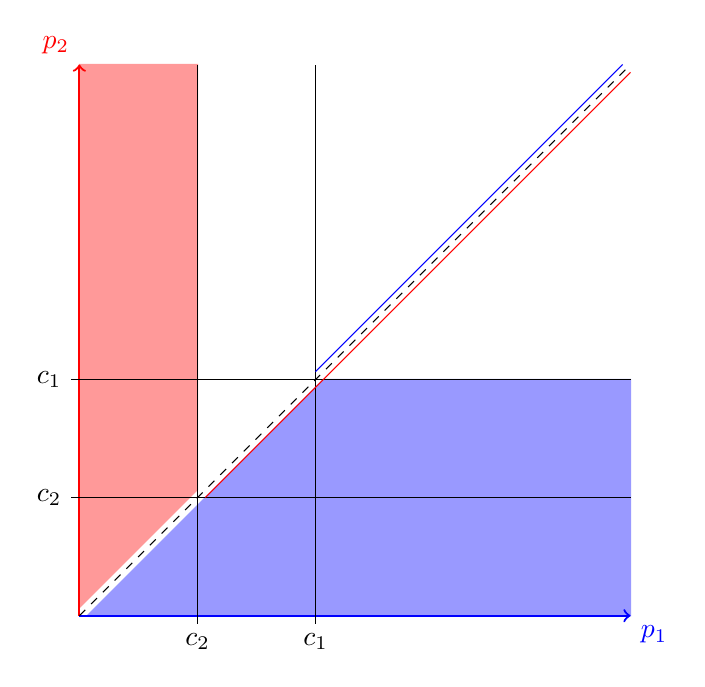
\begin{tikzpicture}[
    dot/.style={shape=circle, inner sep=2pt, draw, node contents=},
    circ/.style={shape=circle, inner sep=2pt, draw, fill}]
    \draw[pattern=north west lines, red!40] (0,0.1) -- (1.5,1.6) -- (1.5,7) -- (0,7) -- cycle;
    \draw[pattern=north west lines, blue!40] (0.1,0) -- (3.1,3) -- (7,3) -- (7,0) -- cycle;
    \draw[thick,blue,->] (0,0) -- (7,0) node[anchor=north west] {$p_1$};
    \draw[thick,red,->] (0,0) -- (0,7) node[anchor=south east] {$p_2$};
    \draw (3pt,1.5cm) -- (-3pt,1.5cm) node[anchor=east] {$c_2$}; 
    \draw (3pt,3cm) -- (-3pt,3cm) node[anchor=east] {$c_1$}; 
    \draw (3cm,3pt) -- (3cm,-3pt) node[anchor=north] {$c_1$};
    \draw (1.5cm,3pt) -- (1.5cm,-3pt) node[anchor=north] {$c_2$};
    \draw[thin] (0,1.5) -- (7,1.5);
    \draw[thin] (3,0) -- (3,7);
    \draw[thin] (1.5,0) -- (1.5,7);
    \draw[thin] (0,3) -- (7,3);
    \draw[dashed] (0,0) -- (7,7);

    \draw[red] (1.6,1.5) -- (7,6.9);
    \draw[blue] (3,3.1) -- (6.9,7);
  \end{tikzpicture}
\end{center}

\subsection*{c)}

The most likely outcome is that Firm 2 sets price at the profit maximizing price
in the range $(c_2, c_1)$. This would then make Firm 1's best response be to
simply not produce (i.e. by setting price below $p_2$), meaning that Firm 2 can make actual profit in this price
range, greater than when they split the market if they charge $p_2 \geq c_1$.

\section*{Problem 3}

\subsection*{a)}

If they cannot price discriminate, then $MR = \frac{d}{dQ}(70 - \frac{1}{2}Q)Q = 70 - Q$.

\subsection*{b)}

The profit maximizing output of the one price monopolist is then $70 - Q = 20
\implies Q = 50 \implies 50 = 140 - 2P \implies P = 45$.

\subsection*{c)}

\begin{center}
  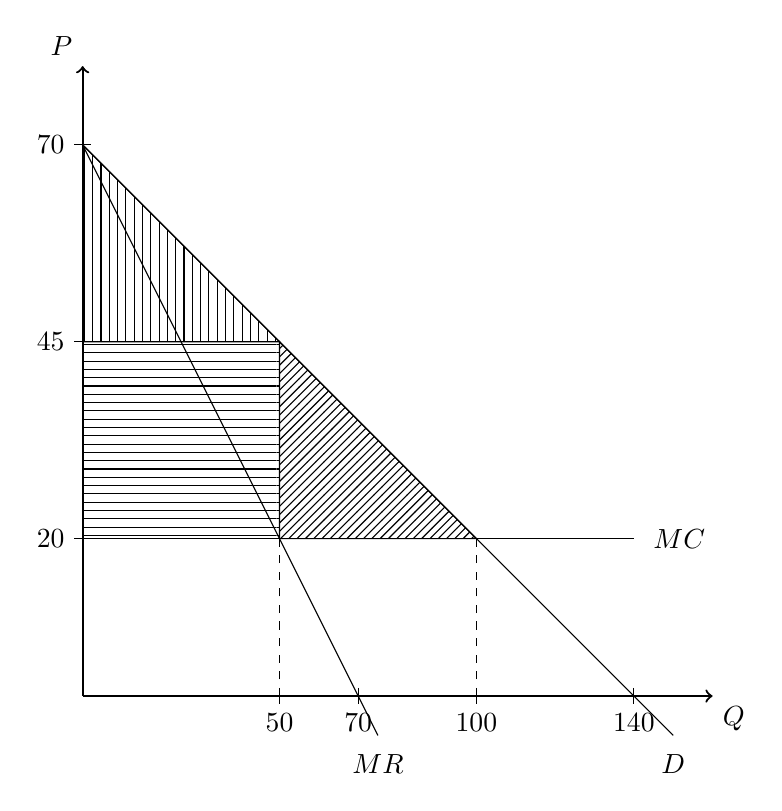
\begin{tikzpicture}[
    dot/.style={shape=circle, inner sep=2pt, draw, node contents=},
    circ/.style={shape=circle, inner sep=2pt, draw, fill}]
    \draw[thick,->] (0,0) -- (8,0) node[anchor=north west] {$Q$};
    \draw[thick,->] (0,0) -- (0,8) node[anchor=south east] {$P$};

    \draw (3pt,7cm) -- (-3pt,7cm) node[anchor=east] {$70$}; 
    \draw (3pt,2cm) -- (-3pt,2cm) node[anchor=east] {$20$}; 
    \draw (3pt,4.5cm) -- (-3pt,4.5cm) node[anchor=east] {$45$}; 
    \draw (7cm,3pt) -- (7cm,-3pt) node[anchor=north] {$140$};
    \draw (2.5cm,3pt) -- (2.5cm,-3pt) node[anchor=north] {$50$};
    \draw (5cm,3pt) -- (5cm,-3pt) node[anchor=north] {$100$};
    \draw (3.5cm,3pt) -- (3.5cm,-3pt) node[anchor=north] {$70$};
    \draw[domain=0:150,scale=0.1,smooth,variable=\x] plot ({\x / 2},{70 - 0.5*\x}) node[label=below:{$D$}]{};
    \draw[domain=0:75,scale=0.1,smooth,variable=\x] plot ({\x / 2},{70 - \x}) node[label=below:{$MR$}]{};
    \draw[domain=0:140,scale=0.1,smooth,variable=\x] plot ({\x / 2},{20}) node[label=right:{$MC$}]{};
    \draw[dashed] (2.5, 0) -- (2.5, 4.5) -- (0, 4.5);
    \draw[dashed] (5,0) -- (5,2);
    \draw[pattern=vertical lines] (0,4.5) -- (0,7) -- (2.5,4.5) -- cycle;
    \draw[pattern=horizontal lines] (0,4.5) -- (2.5,4.5) -- (2.5,2) -- (0,2) -- cycle;
    \draw[pattern=north east lines] (2.5,2) -- (2.5,4.5) -- (5,2) -- cycle;
    % \draw[dashed] (1.5, 1.5) -- (0, 1.5);
    % \draw[dashed] (2.25, 0) -- (2.25, 2.25) -- (0, 2.25);
  \end{tikzpicture}
\end{center}

Consumer surplus (= $\frac{1}{2}(25)(50) = 625$) is in vertical lines, producer
surplus (= $25(50) = 1250$) in horizontal lines, and
deadweight loss (= $\frac{1}{2}(25)(50) = 625$) in northeast lines.


\subsection*{d)}

Players: Incumbent, Entrant

Strategy Sets: Incumbent picks $q_I \geq 0$, Entrant picks $q_E \geq 0$.

Payoffs: Incumbent has profit $\pi_I(q_I,q_E) = (70 - \frac{1}{2}q_I - \frac{1}{2}q_E)q_I - 200 -
20q_I$, Entrant has profit $\pi_E(q_I,q_E) = (70 - \frac{1}{2}q_I - \frac{1}{2}q_E)q_E - 200 - 20q_E$.

\subsection*{e),f)}

The two firms have best response functions given by

\begin{alignat*}{2}
  &&\frac{\partial \pi_I}{\partial q_I} &= 70 -q_I - \frac{1}{2}q_E - 20 = 0\\
  &\implies& q_I &= 50 - \frac{q_E}{2} \\
  &&\frac{\partial \pi_E}{\partial q_E} &= 70 -q_E - \frac{1}{2}q_I - 20 = 0\\
  &\implies& q_E &= 50 - \frac{q_I}{2} \\
  &\implies& q_I &= 50 - \frac{1}{2}(50 - \frac{1}{2}q_I) \\
  && &= 25\frac{4}{3} = \frac{100}{3}\\
  &\implies& q_E &= \frac{100}{3}
\end{alignat*}

\subsection*{g), i)}

\begin{center}
  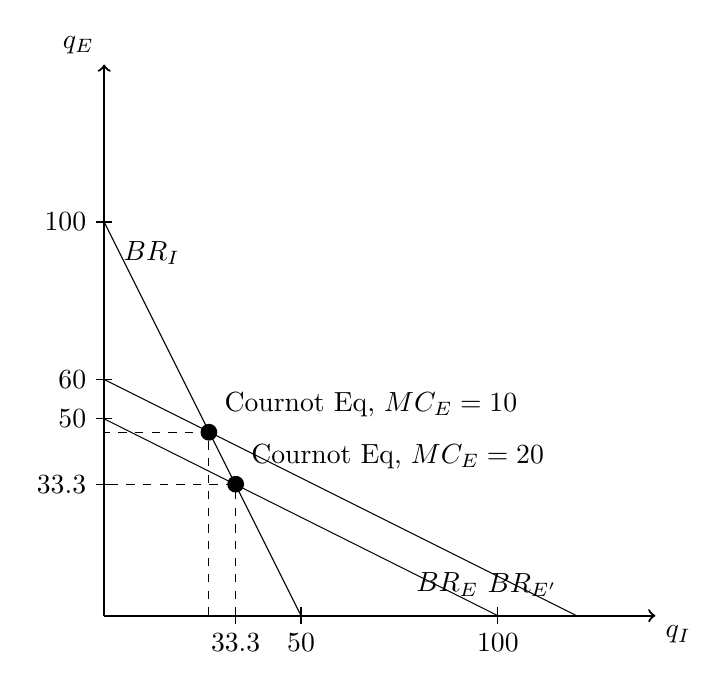
\begin{tikzpicture}[
    dot/.style={shape=circle, inner sep=2pt, draw, node contents=},
    circ/.style={shape=circle, inner sep=2pt, draw, fill}]
    \draw[thick,->] (0,0) -- (7,0) node[anchor=north west] {$q_I$};
    \draw[thick,->] (0,0) -- (0,7) node[anchor=south east] {$q_E$};

    \draw (3pt,5cm) -- (-3pt,5cm) node[anchor=east] {$100$}; 
    \draw (5cm,3pt) -- (5cm,-3pt) node[anchor=north] {$100$};
    \draw (3pt,1.67cm) -- (-3pt,1.67cm) node[anchor=east] {$33.3$}; 
    \draw (1.67cm,3pt) -- (1.67cm,-3pt) node[anchor=north] {$33.3$};
    \draw (3pt,2.5cm) -- (-3pt,2.5cm) node[anchor=east] {$50$}; 
    \draw (3pt,3cm) -- (-3pt,3cm) node[anchor=east] {$60$}; 
    \draw (2.5cm,3pt) -- (2.5cm,-3pt) node[anchor=north] {$50$};
    \draw[domain=0:100,scale=0.05,smooth,variable=\x] plot ({\x},{50 - 0.5*\x}) node[label=above left:{$BR_E$}]{};
    \draw[domain=0:120,scale=0.05,smooth,variable=\x] plot ({\x},{60 - 0.5*\x}) node[label=above left:{$BR_{E'}$}]{};
    \draw[domain=0:100,scale=0.05,smooth,variable=\x] plot ({50 - 0.5*\x},{\x}) node[label=below right:{$BR_I$}]{};

    \draw[dashed] (1.67,0) -- (1.67,1.67) -- (0,1.67);
    \draw[dashed] (1.33,0) -- (1.33,2.33) -- (0,2.33);

    \draw (1.67,1.67) node[circ, label=above right:{Cournot Eq, $MC_E = 20$}]{};
    \draw (1.33,2.33) node[circ, label=above right:{Cournot Eq, $MC_E = 10$}]{};

    % \draw (3pt,4.5cm) -- (-3pt,4.5cm) node[anchor=east] {$45$}; 
    % \draw (7cm,3pt) -- (7cm,-3pt) node[anchor=north] {$140$};
    % \draw (5cm,3pt) -- (5cm,-3pt) node[anchor=north] {$100$};
    % \draw (3.5cm,3pt) -- (3.5cm,-3pt) node[anchor=north] {$70$};
    % \draw[domain=0:140,scale=0.1,smooth,variable=\x] plot ({\x / 2},{20}) node[label=right:{$MC$}]{};
    % \draw[dashed] (2.5, 0) -- (2.5, 4.5) -- (0, 4.5);
    % \draw[dashed] (5,0) -- (5,2);
    % \draw[pattern=vertical lines] (0,4.5) -- (0,7) -- (2.5,4.5) -- cycle;
    % \draw[pattern=horizontal lines] (0,4.5) -- (2.5,4.5) -- (2.5,2) -- (0,2) -- cycle;
    % \draw[pattern=north east lines] (2.5,2) -- (2.5,4.5) -- (5,2) -- cycle;
    % \draw[dashed] (1.5, 1.5) -- (0, 1.5);
    % \draw[dashed] (2.25, 0) -- (2.25, 2.25) -- (0, 2.25);
  \end{tikzpicture}
\end{center}

\subsection*{h)}

The market output is $Q^S = \frac{100}{3} + \frac{100}{3} = \frac{200}{3}$ at a
price of $\frac{200}{3} = 140 - 2P \implies P = \frac{110}{3}$.

\subsection*{h) (again)}

The Entrant's best response function is now given by

\begin{alignat*}{2}
  &&\pi_E(q_I,q_E) &= (70 - \frac{1}{2}q_I - \frac{1}{2}q_E)q_E - 200 - 10q_E \\
  &&\frac{\partial \pi_E}{\partial q_E} &= 70 -q_E - \frac{1}{2}q_I - 10 = 0\\
  &\implies& q_E &= 60 - \frac{q_I}{2} \\
\end{alignat*}

\subsection*{j)}

The Cournot equilibrium is now given by
\begin{alignat*}{2}
  &&\frac{\partial \pi_I}{\partial q_I} &= 70 -q_I - \frac{1}{2}q_E - 20 = 0\\
  &\implies& q_I &= 50 - \frac{q_E}{2} \\
  &&\frac{\partial \pi_E}{\partial q_E} &= 70 -q_E - \frac{1}{2}q_I - 10 = 0\\
  &\implies& q_E &= 60 - \frac{q_I}{2} \\
  &\implies& q_I &= 50 - \frac{1}{2}(60 - \frac{1}{2}q_I) \\
  && &= 20\frac{4}{3} = \frac{80}{3}\\
  &\implies& q_E &= 60 - \frac{1}{2}(50 - \frac{1}{2}q_I) \\
  && &= 35\frac{4}{3} = \frac{140}{3}\\
\end{alignat*}

\subsection*{k)}

The Entrant is unable to run the Incumbent out of business, as the Incumbent
still makes $\pi_I = (70 - \frac{1}{2}(\frac{220}{3}))\frac{80}{3} - 200 -
20\frac{80}{3} = \frac{1400}{9}$.

\end{document}
% LocalWords:  nodecirc
